\documentclass{article}
\usepackage{graphicx}
\graphicspath{{images/}}

\title{
    Usability Test\\
    \begin{large}
      \textit{Web-Application}
    \end{large}
}
\date{
    \begin{small}
        \today
    \end{small}
}
\author{
    Team Recursive Recursion \\
    Retro Rabbit
}

\begin{document}
    %===========================================================================
    % TITLE
    %===========================================================================
    \pagenumbering{gobble}
    \maketitle
    \newpage

    %===========================================================================
    % DOCUMENT
    %===========================================================================
    \pagenumbering{arabic}

    
    \tableofcontents
    \newpage
	\section{Background}    
	\paragraph{}
	The usability test was conducted on the Web-Application. The Web-Application allows a golfcourse owner/manager to map a golfcourse. Our testers played the role of the golfcourse managers to map out a golfcourse. The testers received a few tasks to complete. We (recursive recursion) observed while the testers were busy to gather some valuable information about the Web-Application. The test was conducted in the collaborative labs in the Information Technology building of the University of Pretoria. The test was held on 12 September 2018.


	\section{Methodology}
	\paragraph{•}
	  The participants were friends and acquaintances of the group. The participants all come from different backgrounds and fields of study. The participants were given a brief description of the Web-Application. The test was conducted in a test environment, the participants could not talk to one another and sat far from each other.
	  
	  \section{Pictures of the test}
	  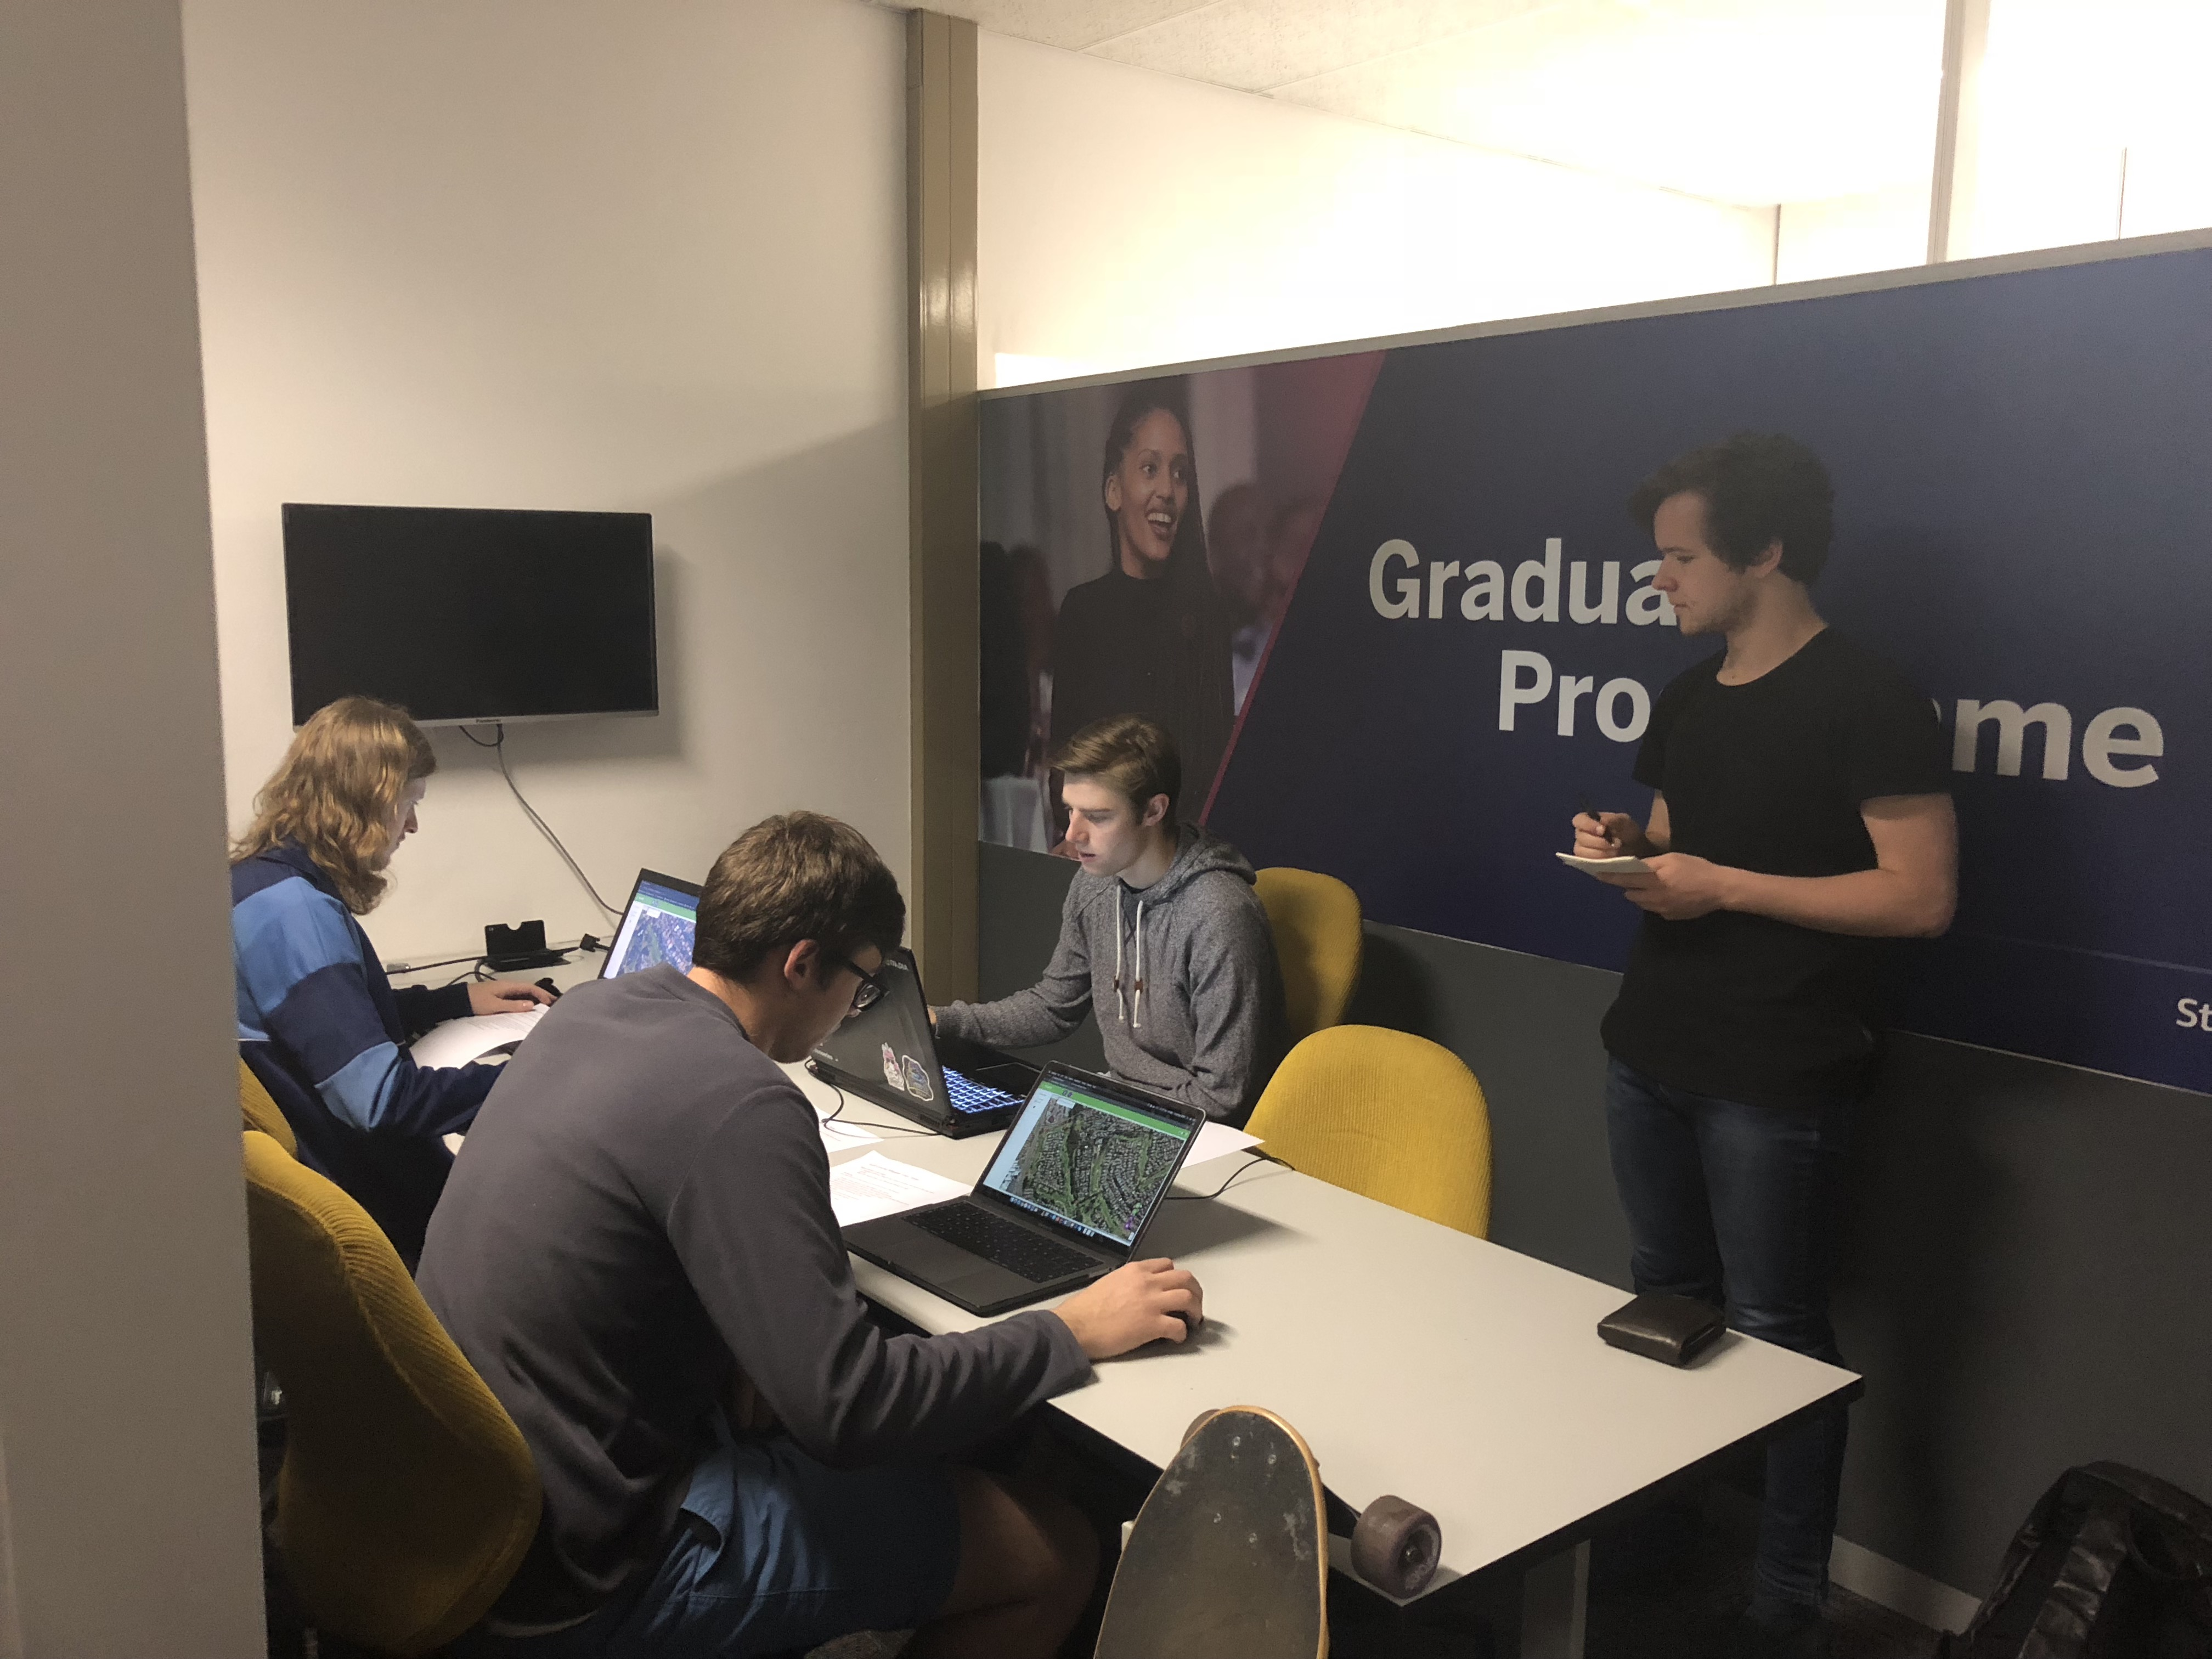
\includegraphics[scale=0.1]{img}
	  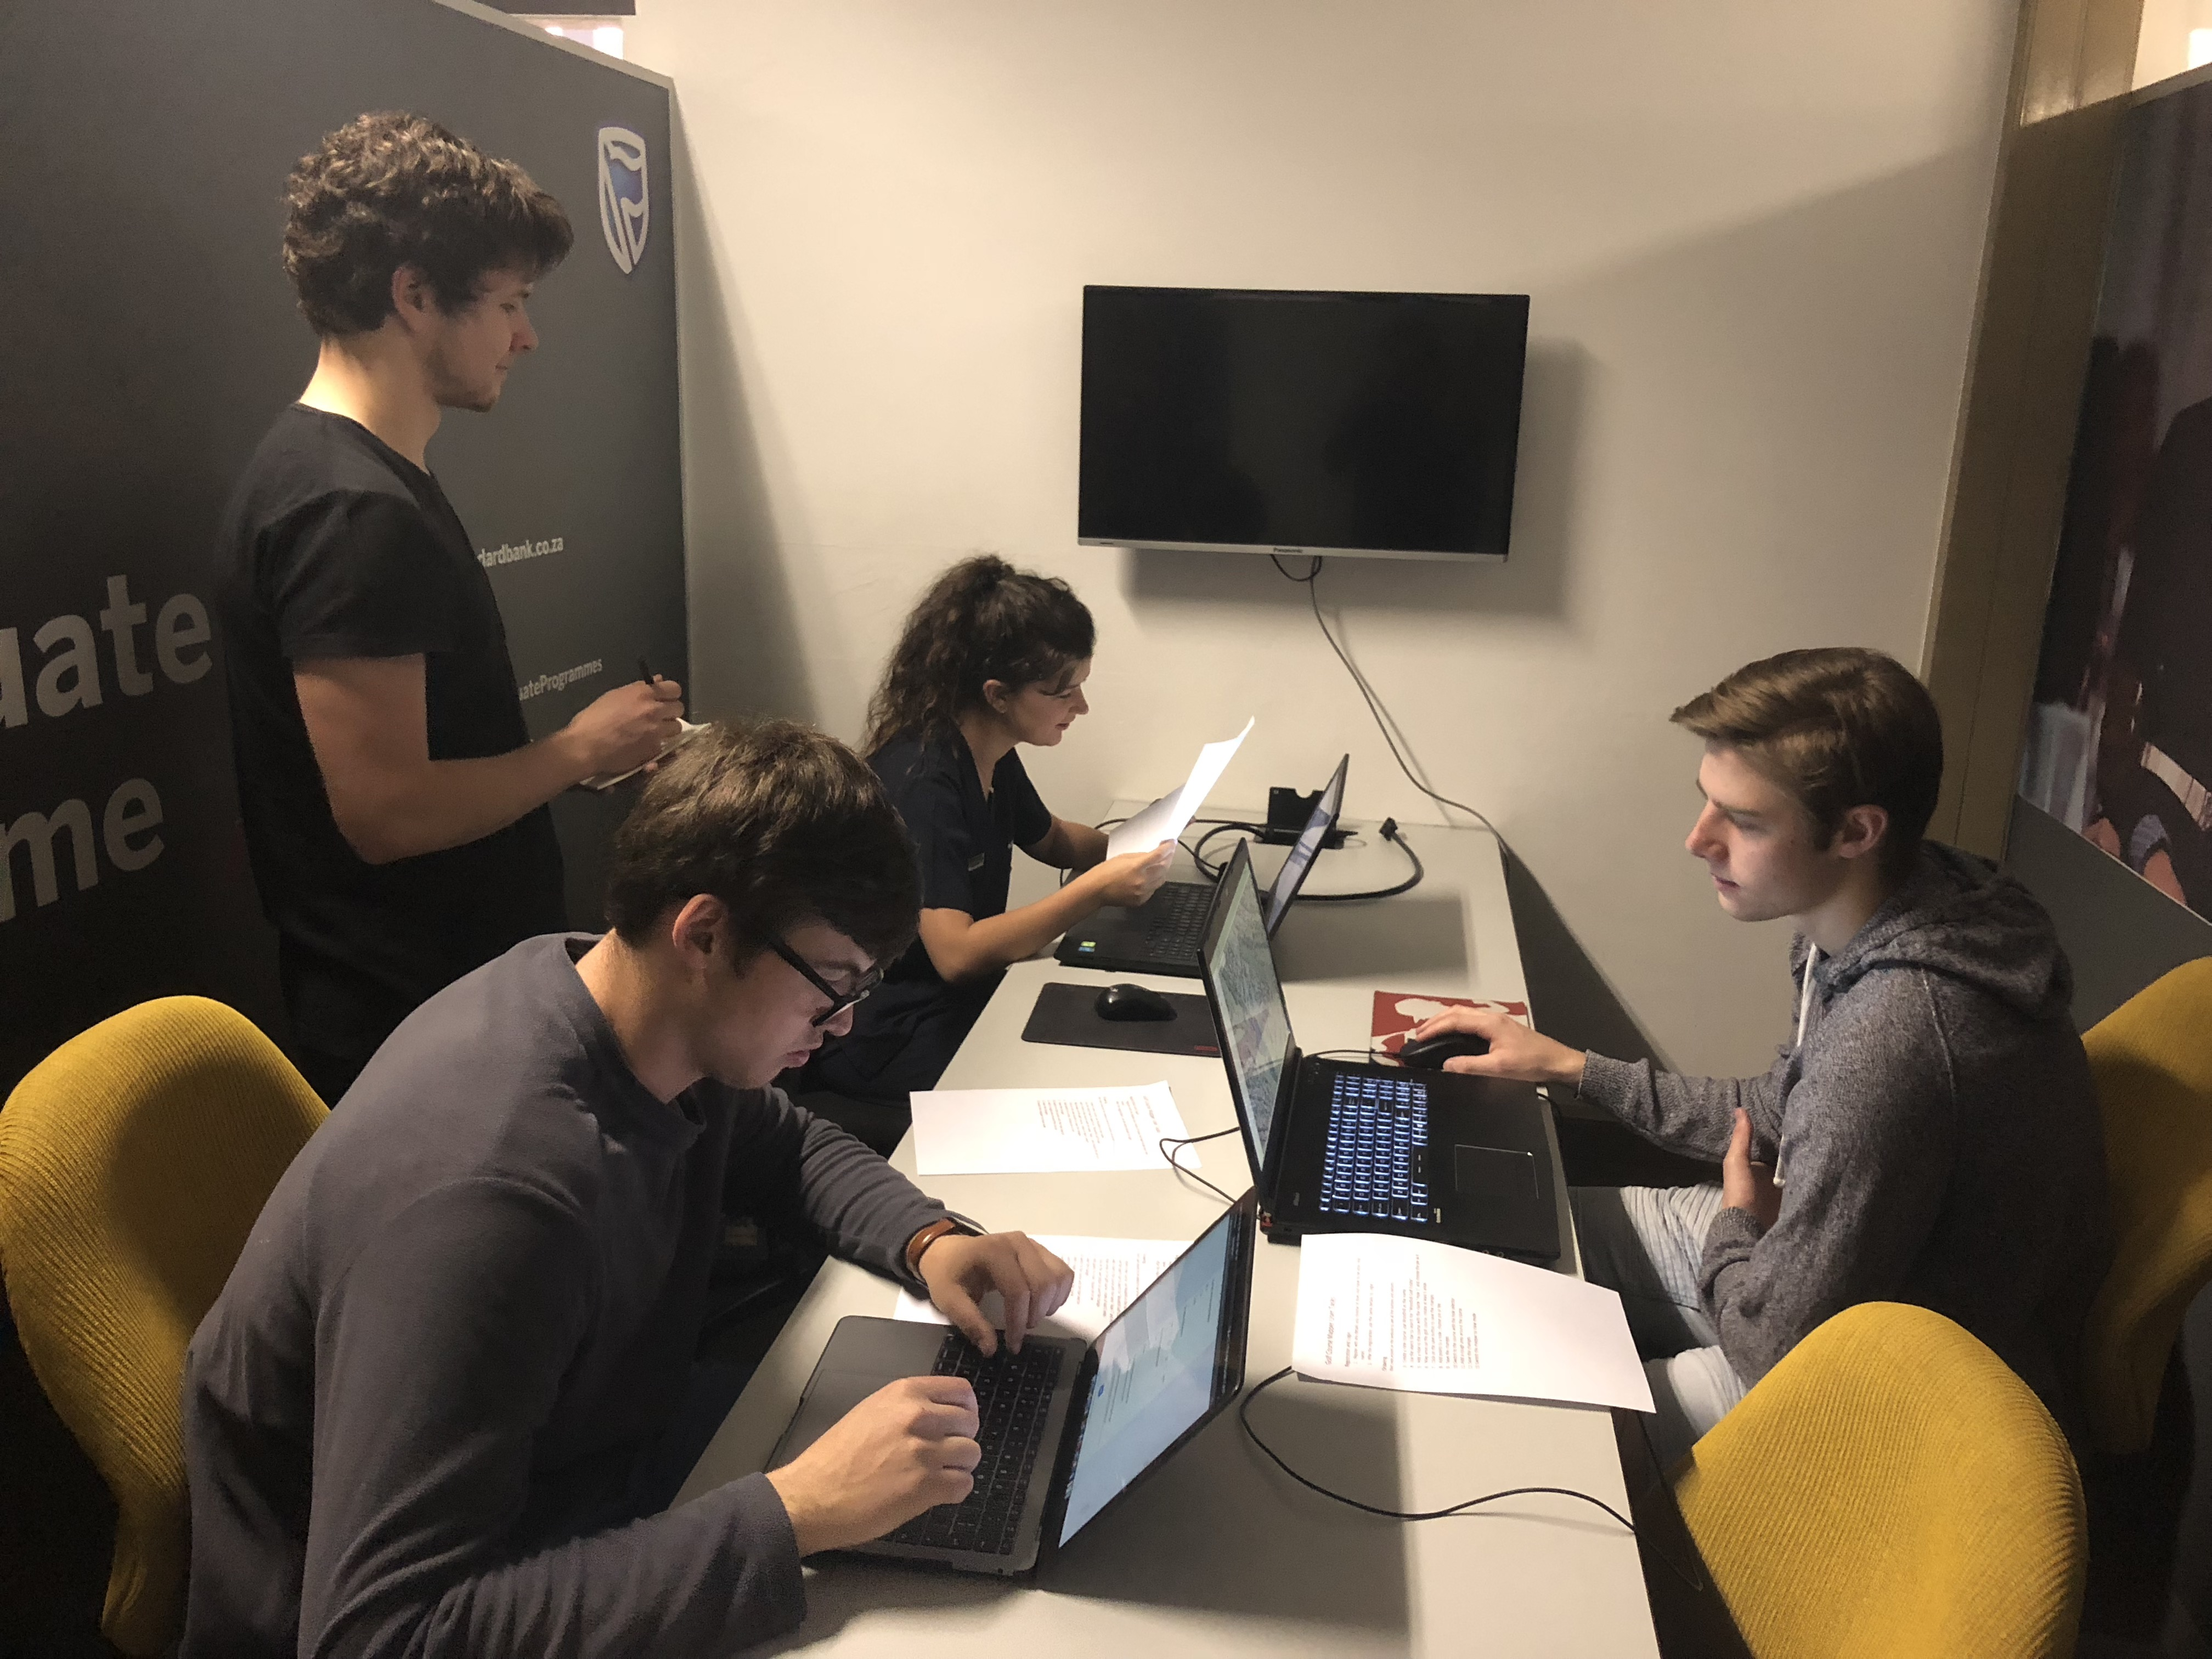
\includegraphics[scale=0.1]{img2}
	
	\section{Test Results}
	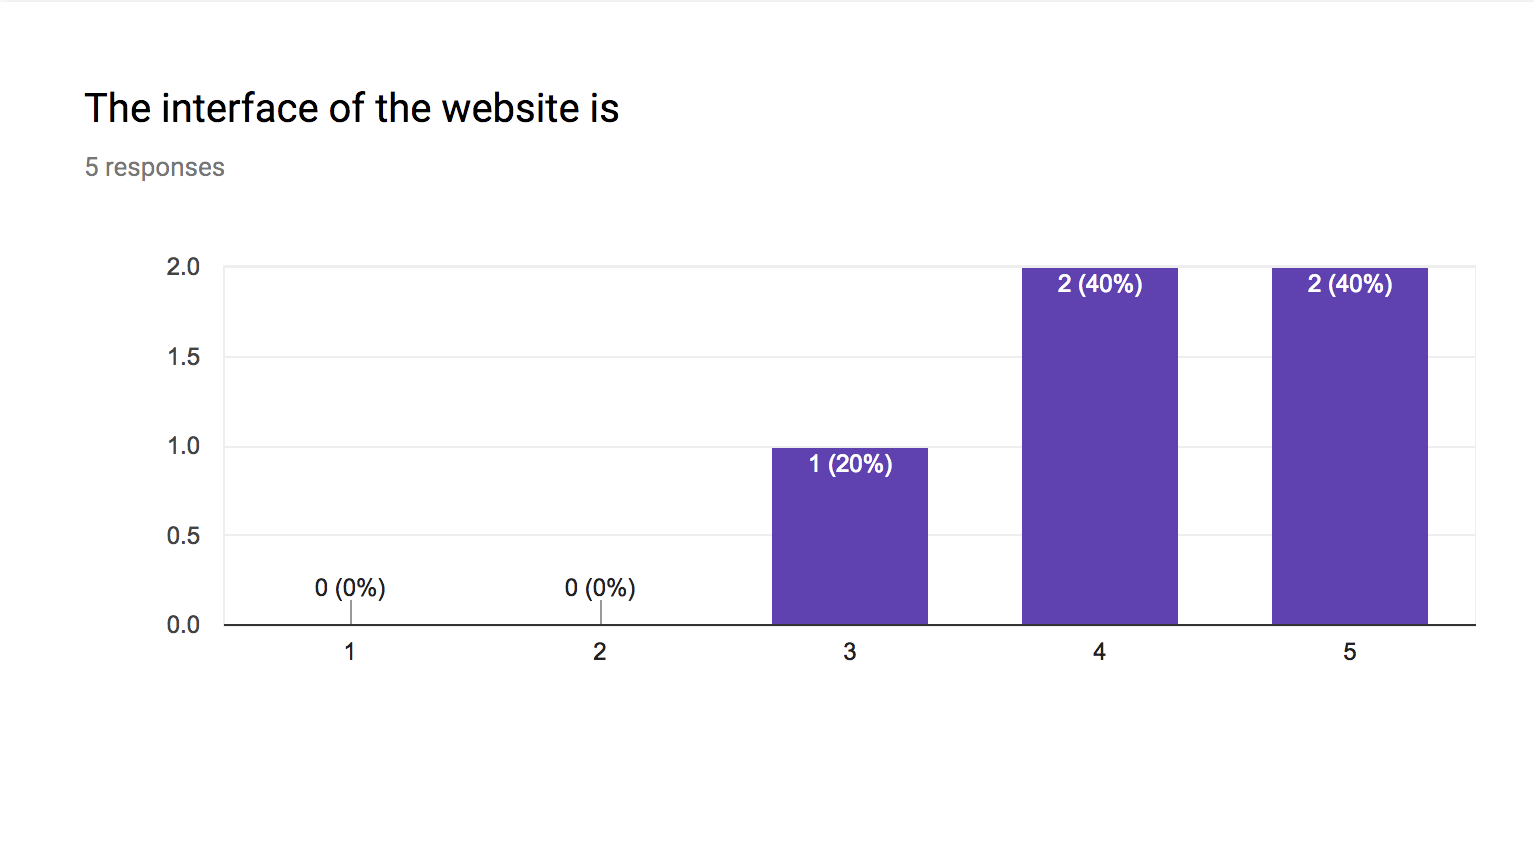
\includegraphics[scale=0.5]{g1}
	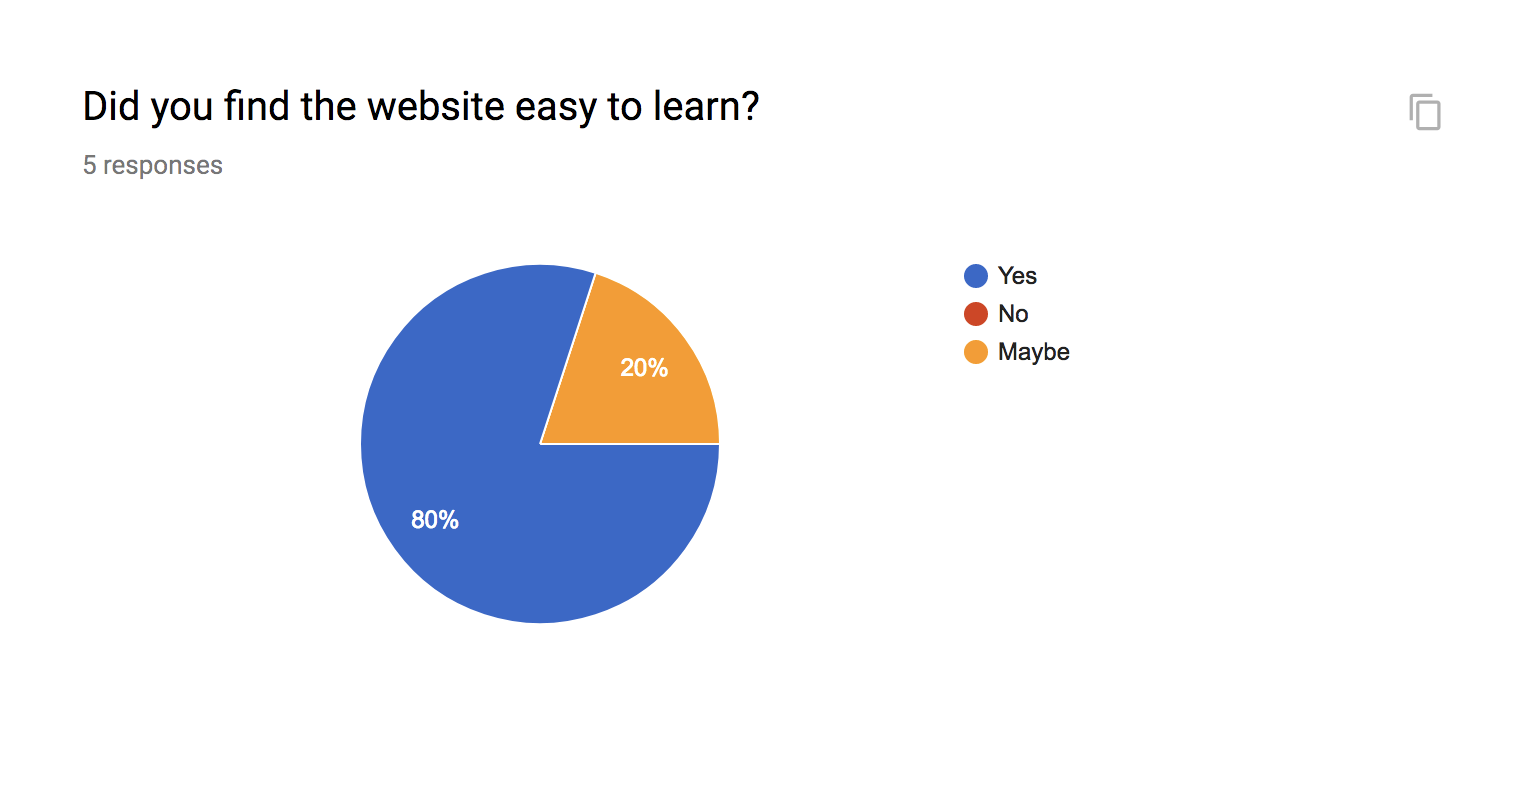
\includegraphics[scale=0.5]{g2}
	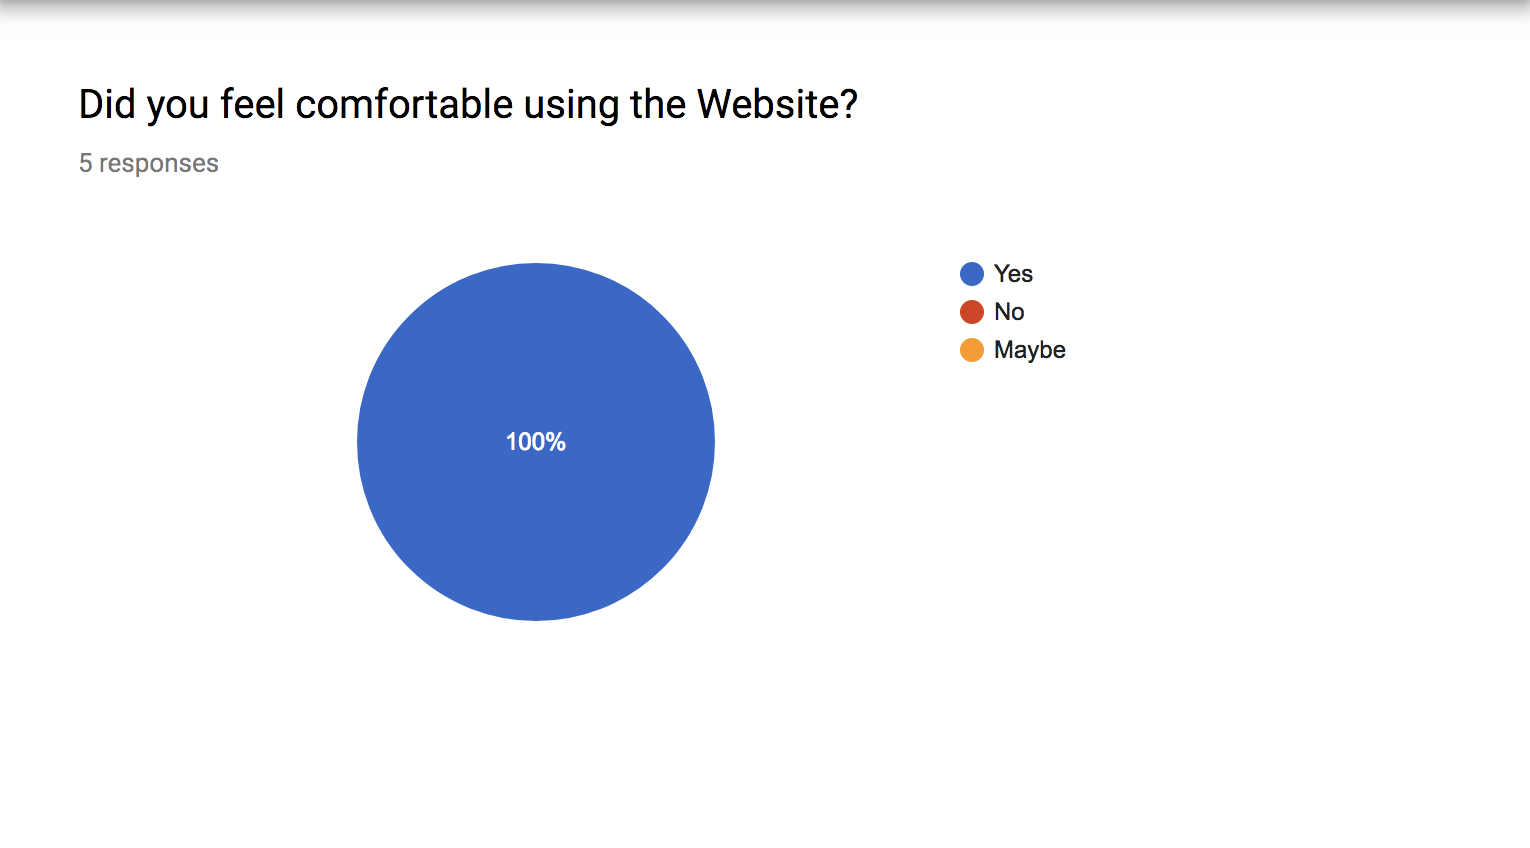
\includegraphics[scale=0.5]{g3}
	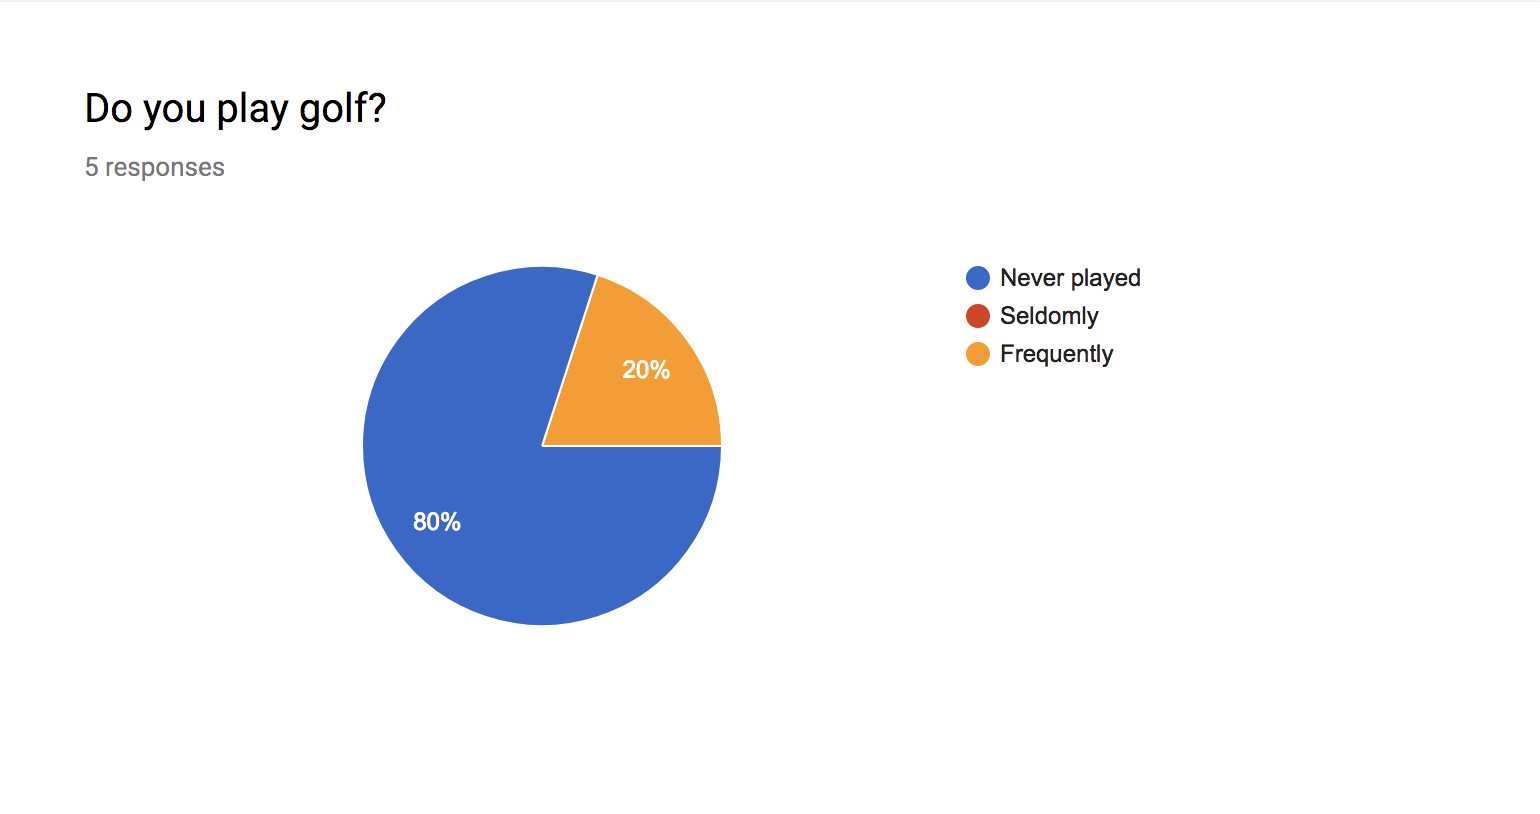
\includegraphics[scale=0.5]{g4}
	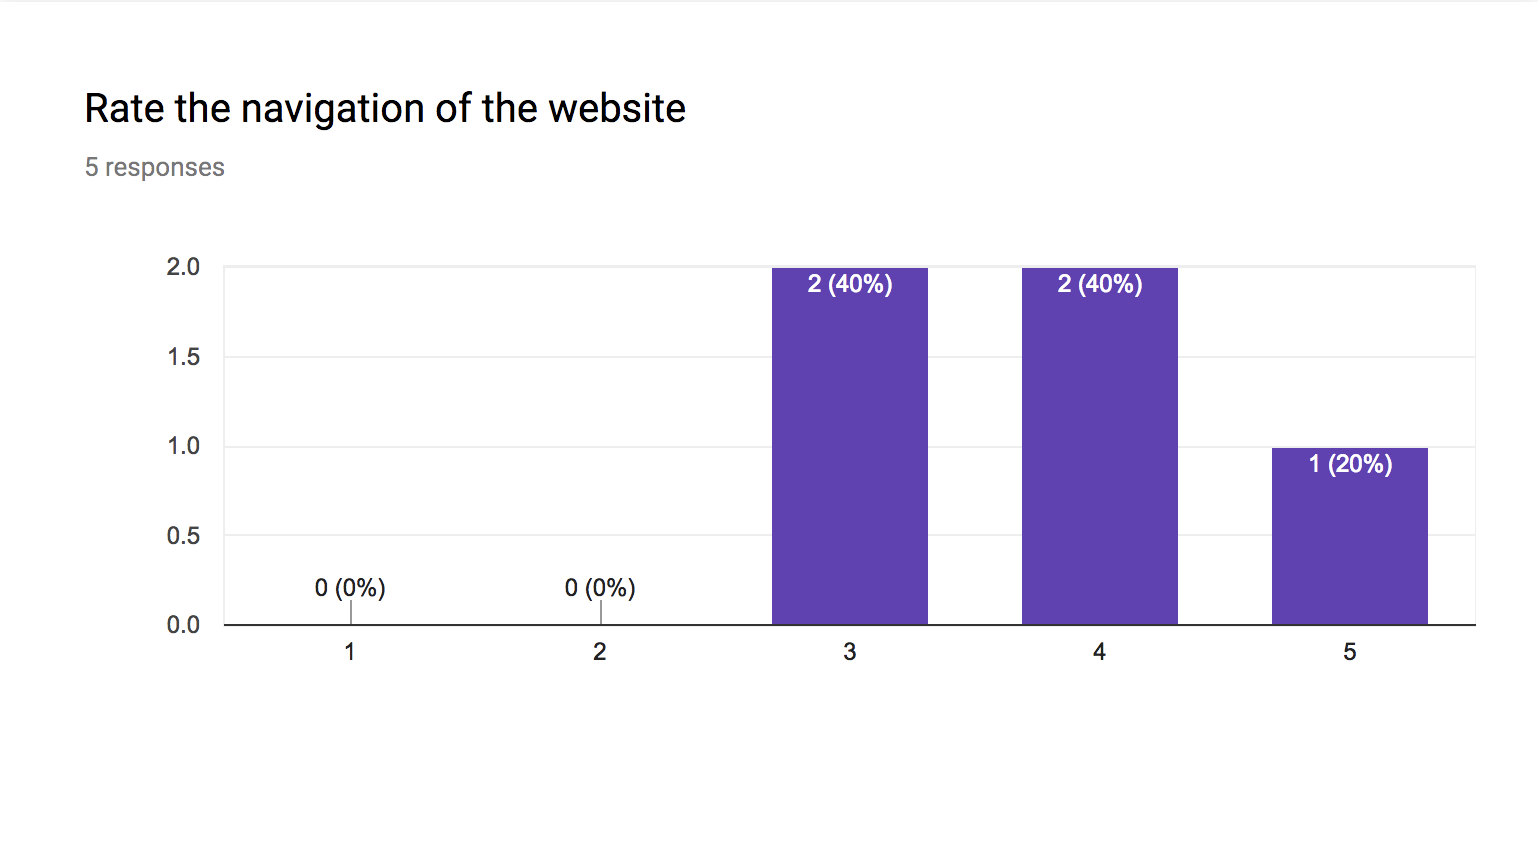
\includegraphics[scale=0.5]{g5}
	
	\paragraph{•}
	By observing the participants while they were busy we gained valuable information about the interface, especially how the interface is organized. We made minor changes to make the Web-Application easier to use. 
	
	\section{Findings and Recommendations}
	\paragraph{•}
	We made minor changes to the interface, such as reorganizing the elements of the interface. We also added a help section to the landing page of the Web-Application. There is also a YouTube tutorial on the landing page to help learn how to use the Web-Application.
	
	

	
	

	
	
\end{document}